\section{A Wait-Free Method for Top-Down BFS}
\label{sec:wf-topdown}

This section presents our method with top-down steps only; Section~\ref{sec:dir-opt} adds bottom-up steps. In place of the barrier that ends a level, every thread decides on its own when a level is complete, and finishes any part of it that the others have left undone (Figure~\ref{fig:td-protocol}). Algorithm~\ref{alg:wf-td} gives the method as thread $t$ runs it.

\begin{figure*}
    \centering
    \begin{tikzpicture}[protocol]
        \draw[lane] (1.85,1.5) -- (16.45,1.5);
        \draw[lane] (1.85,0) -- (16.45,0);
        \node[anchor=east, align=right] at (1.75,1.5) {thread $t$,\\ owner of $u$};
        \node[anchor=east, align=right] at (1.75,0) {thread $h$,\\ a helper};
        % thread t expands u, a vertex of its own bucket
        \node[work] (o1) at (2.55,1.5) {append $v$};
        \node[cert] (o2) at (4.1,1.5) {$\mathit{dist}[v] \gets d{+}1$};
        \node[note, below=2pt of o2] {after\\ the append};
        \draw[stall] (5.1,1.5) -- (12.55,1.5);
        \node[note, anchor=south] at (8.8,1.62) {reads $\mathit{dist}[w] = -1$, then stalls before it appends $w$};
        \node[late] (o3) at (13.45,1.5) {append $w$};
        \node[late] (o4) at (15.05,1.5) {$\mathit{dist}[w] \gets d{+}1$};
        \node[note, anchor=south] at (14.25,1.78) {late, but harmless};
        % thread h takes over what t left of its bucket
        \node[note] (h0) at (5.05,0) {expands $u$;\\ $v$ is discovered};
        \node[work] (h1) at (6.5,0) {append $w$};
        \node[cert] (h2) at (8.2,0) {$\mathit{dist}[w] \gets d{+}1$};
        \node[cert] (h3) at (10.15,0) {set $\mathit{expanded}[u]$};
        \node[cert] (h4) at (11.85,0) {set $\mathit{done}_{d,t}$};
        \node[note, below=2pt of h2] {after\\ the append};
        \node[note, below=2pt of h3] {after every\\ neighbor};
        \node[note, below=2pt of h4] {after\\ the bucket};
        \draw[->] (12.55,0) -- (16.45,0) node[note, pos=0.55, above=2pt] {goes on to level $d{+}1$, where it expands $w$};
        % the level is complete before t resumes
        \draw[densely dashed, gray] (12.7,-0.85) -- (12.7,2.2) node[note, above] {level $d$ complete};
        % key
        \node[key, work] at (2.1,-1.4) {};
        \node[note, anchor=west] at (2.4,-1.4) {work};
        \node[key, cert] at (3.4,-1.4) {};
        \node[note, anchor=west] at (3.7,-1.4) {a write that lets other threads skip the work before it};
        \node[key, late] at (10.0,-1.4) {};
        \node[note, anchor=west] at (10.3,-1.4) {a late write};
        \draw[stall] (11.85,-1.4) -- (12.4,-1.4);
        \node[note, anchor=west] at (12.55,-1.4) {stalled};
    \end{tikzpicture}
    \caption{Helping in a top-down level $d$, with two threads. Thread $t$ stalls while it expands a vertex $u$ of its own bucket, after it reads $\mathit{dist}[w] = -1$. Thread $h$, helping with the rest of that bucket, finds $u$ past $\mathit{last}_{d,t}$ and $\mathit{expanded}[u]$ unset, expands $u$ again, appends $w$, and sets $\mathit{expanded}[u]$ and $\mathit{done}_{d,t}$. The late writes of $t$ when it resumes are harmless (Section~\ref{sec:td-order}).}
    \Description{A timeline of two threads in one level. The owner appends a neighbor and sets its distance, then stalls; the helper expands the same vertex, appends the other neighbor, sets its distance, marks the vertex and the owner's bucket finished, and moves on to the next level; the owner resumes afterwards and repeats the append and the distance, which changes nothing.}
    \label{fig:td-protocol}
\end{figure*}

\subsection{Levels and Buckets}
\label{sec:td-structure}

The levels of a search form a linked list, whose node $N_d$ describes level $d$ (Figure~\ref{fig:td-example}). A node holds its depth $d$, a pointer $\mathit{next}$ to the node of level $d+1$, which is null until some thread links that node, and one \emph{entry} for each thread. Entry $t$ of $N_d$ holds the \emph{bucket} $B_{d,t}$, a list of vertices of level $d$ that thread $t$ has discovered, and two fields that record how far the expansion of the bucket has got: $\mathit{last}_{d,t}$, the position of the last vertex of $B_{d,t}$ that thread $t$ itself has finished, which starts at $-1$, and the flag $\mathit{done}_{d,t}$, which a thread sets once it has finished the vertices of the bucket. Only thread $t$ appends to $B_{d,t}$, and only thread $t$ writes $\mathit{last}_{d,t}$.

Besides the distances, the method keeps a flag $\mathit{expanded}[u]$ for every vertex $u$: a thread sets it once it has examined every neighbor of $u$, and other threads then skip $u$. A vertex can be in several buckets of a level, since several threads can discover it at the same time, but every copy is in the right level: a vertex in $B_{d,t}$ is at distance $d$. Before a search, as Section~\ref{sec:bg-method} requires, $N_0$ holds the source $s$ in the bucket of thread $0$ and every other bucket of $N_0$ is empty, every $\mathit{last}$ is $-1$, every flag $\mathit{done}$ and $\mathit{expanded}$ is unset, $N_0.\mathit{next}$ is null, $\mathit{dist}[s] = 0$, and every other distance is $-1$.

\begin{algorithm}
\caption{Wait-free top-down BFS, as thread $t$ runs it. For a node $N = N_d$, $N.B[o]$, $N.\mathit{last}[o]$ and $N.\mathit{done}[o]$ stand for $B_{d,o}$, $\mathit{last}_{d,o}$ and $\mathit{done}_{d,o}$.}
\label{alg:wf-td}
\begin{algorithmic}[1]
\Procedure{BFS}{$s$}
    \State $N \gets N_0$
    \While{$N \neq \mathit{null}$}
        \State \textbf{fence} \label{ln:td-fence}
        \State \Call{ExpandLevel}{$N$}
        \State $N \gets N.\mathit{next}$ \label{ln:td-next}
    \EndWhile
\EndProcedure
\Statex
\Procedure{ExpandLevel}{$N$}
    \State $\rho \gets t$, then the other threads in a random order \label{ln:td-order}
    \For{$k \gets 0$ \textbf{to} $T-1$}
        \State $o \gets \rho[k]$
        \IfThen{$N.\mathit{done}[o]$ \textbf{or} $N.B[o]$ is empty}{\textbf{continue}}
        \IfThen{$N.\mathit{next} = \mathit{null}$}{\Call{AddLevel}{$N$}} \label{ln:td-add}
        \State $\mathit{size} \gets N.B[o].\mathit{size}$; $A \gets N.B[o].\mathit{array}$ \label{ln:td-size}
        \If{$o = t$}
            \For{$i \gets 0$ \textbf{to} $\mathit{size}-1$} \label{ln:td-own}
                \State \Call{Expand}{$N$, $A[i]$}
                \State $N.\mathit{last}[t] \gets i$ \label{ln:td-last}
            \EndFor
        \Else
            \State $\mathit{first} \gets N.\mathit{last}[o] + 1$ \label{ln:td-first}
            \ForAll{$i$ from $\mathit{first}$ to $\mathit{size}-1$, in a random order} \label{ln:td-help}
                \State \Call{Expand}{$N$, $A[i]$}
            \EndFor
        \EndIf
        \State $N.\mathit{done}[o] \gets \mathit{true}$ \label{ln:td-done}
    \EndFor
\EndProcedure
\Statex
\Procedure{Expand}{$N$, $u$}
    \IfThen{$\mathit{expanded}[u]$}{\textbf{return}}
    \ForAll{neighbors $v$ of $u$, in the order of Section~\ref{sec:td-contention}} \label{ln:td-nbrs}
        \If{$\mathit{dist}[v] = -1$}
            \State append $v$ to $N.\mathit{next}.B[t]$ \label{ln:td-push}
            \State $\mathit{dist}[v] \gets N.\mathit{depth} + 1$ \label{ln:td-dist}
        \EndIf
    \EndFor
    \State $\mathit{expanded}[u] \gets \mathit{true}$ \label{ln:td-expanded}
\EndProcedure
\Statex
\Procedure{AddLevel}{$N$}
    \State $M \gets$ the spare node of $t$, or a new node
    \State $M.\mathit{depth} \gets N.\mathit{depth} + 1$
    \State $\mathit{linked} \gets$ \Call{CAS}{$N.\mathit{next}$, $\mathit{null}$, $M$} \label{ln:td-cas}
    \State the spare node of $t$ becomes null if $\mathit{linked}$, and $M$ if not
\EndProcedure
\end{algorithmic}
\end{algorithm}

\subsection{An Example}
\label{sec:td-example}

\begin{figure}
    \centering
    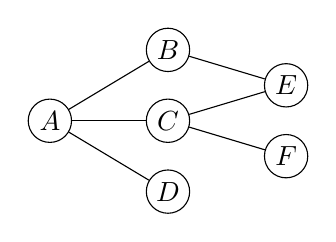
\begin{tikzpicture}[vertex/.style={circle, draw, minimum size=0.55cm, inner sep=0pt}]
        \node[vertex] (A) at (0,0) {$A$};
        \node[vertex] (B) at (1.5,0.9) {$B$};
        \node[vertex] (C) at (1.5,0) {$C$};
        \node[vertex] (D) at (1.5,-0.9) {$D$};
        \node[vertex] (E) at (3,0.45) {$E$};
        \node[vertex] (F) at (3,-0.45) {$F$};
        \draw (A) -- (B);
        \draw (A) -- (C);
        \draw (A) -- (D);
        \draw (B) -- (E);
        \draw (C) -- (E);
        \draw (C) -- (F);
    \end{tikzpicture}

    \vspace{0.3cm}

    \begin{tikzpicture}[>=Stealth, levelnode/.style={draw, rectangle, align=left, font=\footnotesize, minimum width=1.55cm, inner sep=3pt}]
        \node[levelnode] (n0) at (0,0) {$N_0$\\ $0$: $A$\\ $1$: --};
        \node[levelnode] (n1) at (2.05,0) {$N_1$\\ $0$: $B, C$\\ $1$: $C, D$};
        \node[levelnode] (n2) at (4.1,0) {$N_2$\\ $0$: $E$, \textcolor{gray}{$F^{\ast}$}\\ $1$: $F$};
        \node[levelnode] (n3) at (6.15,0) {$N_3$\\ $0$: --\\ $1$: --};
        \draw[->] (n0) -- (n1);
        \draw[->] (n1) -- (n2);
        \draw[->] (n2) -- (n3);
    \end{tikzpicture}
    \caption{A search from $A$ with two threads; each node lists the buckets of threads $0$ and $1$. Thread $0$ appends the gray $F^{\ast}$ after thread $1$ has finished the search.}
    \Description{A graph with vertices A to F, and the four level nodes of a search from A by two threads, with the buckets of each thread in each node.}
    \label{fig:td-example}
\end{figure}

Figure~\ref{fig:td-example} shows a search from $A$ with two threads. Thread 1, whose bucket of level 0 is empty, helps thread 0 with $A$, and both discover $C$, so level 1 holds it twice. In level 1, thread 0 reads $\mathit{dist}[F] = -1$ while it expands $C$, and stalls; thread 1 expands its own bucket, which discovers $F$, finds the rest of the bucket of thread 0 expanded, expands level 2, finds the buckets of $N_3$ empty, and returns. The search is complete although thread 0 is still stalled; when it resumes, it appends $F$ to $B_{2,0}$, a late copy that changes nothing (Section~\ref{sec:td-order}).

\subsection{Expanding a Level}
\label{sec:td-expand}

A thread expands level $d$ by visiting the $T$ entries of $N_d$, its own first and then those of the other threads in a random order, drawn anew for every level (\textsc{ExpandLevel}, line~\ref{ln:td-order}). It skips an entry whose bucket is empty or whose flag $\mathit{done}$ is set; otherwise it reads the size of the bucket, expands the vertices before that position, and sets $\mathit{done}$. In its own bucket, it expands the vertices in order, publishing its position in $\mathit{last}_{d,t}$ after each (line~\ref{ln:td-last}); in the bucket of another thread $o$, it expands only the vertices after position $\mathit{last}_{d,o}$, which $o$ had not finished when the helper read it, in a random order (line~\ref{ln:td-help}). Expanding a vertex $u$ does nothing if $\mathit{expanded}[u]$ is set (\textsc{Expand}); otherwise, the thread appends every neighbor $v$ with $\mathit{dist}[v] = -1$ to its own bucket in $N_{d+1}$ and sets $\mathit{dist}[v] = d+1$, and sets $\mathit{expanded}[u]$ once it has examined every neighbor (line~\ref{ln:td-expanded}).

A level is thus an instance of Certified Write-All (Section~\ref{sec:bg-doall}) whose tasks are the positions of the $T$ buckets of $N_d$, to which their owners may still be appending while the others work through them; since $\mathit{done}$ certifies all of a bucket that a thread has read, a thread certifies the whole level for itself by reading $T$ flags, with no pass over the $n$ vertices.

When a thread has visited all $T$ entries of $N_d$, every vertex of level $d$ has been expanded, by it or by another thread, so every vertex of level $d+1$ is in some bucket of $N_{d+1}$, and the thread moves on to $N_{d+1}$ without waiting (line~\ref{ln:td-next}). Before it reads the buckets of the new level, it executes a fence (line~\ref{ln:td-fence}): under TSO, its last appends to $N_{d+1}$ could otherwise still sit in its store buffer, where only it sees them, while others read those buckets (Section~\ref{sec:pf-tso}). Slower threads may still be expanding level $d$; Section~\ref{sec:td-order} explains why they cannot harm the levels after it.

\subsection{The Order of Writes}
\label{sec:td-order}

Threads skip work on the strength of what others have written: a vertex whose distance is set is not discovered again, one whose flag $\mathit{expanded}$ is set is not expanded again, helpers skip the positions up to $\mathit{last}_{d,o}$ of a bucket, and no thread visits a bucket whose flag $\mathit{done}$ is set. We call a write that lets other threads skip work a \emph{certificate}, and the method rests on one rule, which Lemma~\ref{lem:certs} proves for each of them: \emph{every certificate comes after the work that it certifies}. A thread that stops between any two of its steps therefore leaves no work undone that others would skip:
\begin{itemize}
    \item Since a thread appends $v$ to its bucket before it sets $\mathit{dist}[v]$ (lines~\ref{ln:td-push} and~\ref{ln:td-dist}), one that stops in between leaves $\mathit{dist}[v] = -1$, and another thread discovers $v$ again. In the other order, a thread that stopped in between would leave $v$ discovered but in no bucket, and no thread would ever expand it.
    \item A thread that stops in the middle of a vertex $u$ leaves $\mathit{expanded}[u]$ unset (line~\ref{ln:td-expanded}), so others expand $u$ again; they examine the neighbors that it discovered, but do not append them.
    \item $\mathit{last}_{d,t} = i$ follows the expansion of the vertex at position $i$, and $\mathit{done}$ that of every vertex that the thread read in the bucket (lines~\ref{ln:td-last} and~\ref{ln:td-done}).
\end{itemize}
Figure~\ref{fig:td-protocol} shows these orders at work, for a thread that stops between appending one neighbor and the next.
Every thread that discovers $v$ writes the same distance, $d+1$, so the write needs no CAS. Section~\ref{sec:dir-opt} replaces the store with a CAS, so that the direction rule counts the edges of each vertex only once.

A delayed thread can also resume long after the others have moved on. Suppose thread $t$ stopped while expanding a vertex $u$ of level $d$, after it read $\mathit{dist}[w] = -1$ for a neighbor $w$ but before it appended $w$. Before any thread could finish level $d$, some thread finished expanding $u$, and so either appended $w$ or found it discovered, and therefore appended, by another. When $t$ resumes, it appends $w$ to $B_{d+1,t}$, which the others may have expanded already, and writes $\mathit{dist}[w] = d+1$ again: the distance is the one already there, and the late copy of $w$ duplicates one that the others have expanded or will expand, so a thread that read $B_{d+1,t}$ before the late append missed nothing. Such late appends are also why a vertex can have several copies in a level, and why $\mathit{done}$ means that the vertices a thread read in a bucket are finished, not every vertex the bucket will ever hold.

\subsection{Buckets}
\label{sec:td-buckets}

A bucket has to let its owner append vertices, even long after other threads have read it and moved on, while any number of helpers read it by position, without locks, and without ever letting a reader see a position that has not been written or memory that has been freed. It is a dynamic array that only its owner writes (Algorithm~\ref{alg:bucket}), so appends need no CAS.

\begin{algorithm}
\caption{Appending to a bucket $B$, which only its owner does, and reading it, which any thread can do.}
\label{alg:bucket}
\begin{algorithmic}[1]
\Procedure{Append}{$B$, $v$}
    \If{$B.\mathit{size} = B.\mathit{capacity}$}
        \State $c \gets \max(2 \cdot B.\mathit{capacity}, c_0)$
        \State $A \gets$ an array of $c$ vertices from the owner's arena
        \State copy $B.\mathit{array}[0], \ldots, B.\mathit{array}[B.\mathit{size}-1]$ into $A$
        \State $B.\mathit{array} \gets A$ \label{ln:bk-array}
        \State $B.\mathit{capacity} \gets c$
    \EndIf
    \State $B.\mathit{array}[B.\mathit{size}] \gets v$
    \State $B.\mathit{size} \gets B.\mathit{size} + 1$ \label{ln:bk-size}
\EndProcedure
\Statex
\Procedure{Read}{$B$}
    \State $k \gets B.\mathit{size}$
    \State $A \gets B.\mathit{array}$
    \State \Return $A$ and $k$ \Comment{the reader then reads $A[0], \ldots, A[k-1]$ in place}
\EndProcedure
\end{algorithmic}
\end{algorithm}

When the array is full, the owner copies the vertices into one twice as large from its arena, or of a small fixed size $c_0$ at first, and only then publishes it in $\mathit{array}$ (line~\ref{ln:bk-array}); it writes each vertex before it increases $\mathit{size}$ (line~\ref{ln:bk-size}), and only it reads $\mathit{capacity}$. A reader reads in the opposite order, $\mathit{size}$ and then $\mathit{array}$ (Algorithm~\ref{alg:wf-td}, line~\ref{ln:td-size}), and then the positions before that size, in place. The array that it finds is then the one that was current when that size was published, or a later one, which holds copies of the same vertices (Lemma~\ref{lem:buckets}). A reader can miss vertices appended after it read the size, but by the time a thread reads the buckets of $N_d$, every vertex of level $d$ is in them already, and the appends that come later are late copies (Section~\ref{sec:td-order}).

A replaced array cannot be freed during the search, since a delayed reader may hold its pointer for any length of time; it stays in the owner's arena, which is reset once every call has returned. Since capacities double, the old arrays of a bucket hold fewer positions than its current one, so a bucket of $k$ vertices that has outgrown its first array takes fewer than $4k$ positions in all; an append takes constant time amortized, and a growth copies at most $n$ vertices, since a thread appends each vertex at most once in a search (Lemma~\ref{lem:once}).

\subsection{Linking Levels and Ending the Search}
\label{sec:td-link}

A thread that finds a bucket of $N_d$ to expand first makes sure that $N_{d+1}$ exists, since its discoveries go there (line~\ref{ln:td-add}): if $N_d.\mathit{next}$ is null, it prepares a node and tries to link it with a CAS from null (line~\ref{ln:td-cas}), and if the CAS fails, it uses the node that another thread linked. A node that lost the race was never seen by another thread, so its thread keeps it as a spare for the next level; threads tend to reach a level together, so without spares most of the nodes they prepare would be wasted.

$N_{d+1}$ is linked before any thread expands a vertex of level $d$ or sets a flag $\mathit{done}$, so a thread that skips a done bucket still finds $N_{d+1}$ linked. A level without vertices gets no successor: no thread links a node after it, and every thread that visits it finds $\mathit{next}$ null and returns (line~\ref{ln:td-next}). The first such level is level $D+1$, so every call goes through the nodes of levels $0$ to $D+1$ and returns there.

\subsection{Keeping Helpers Apart}
\label{sec:td-contention}

The method is correct whatever order the threads take entries and neighbors in, and helpers take positions in; the orders we use keep the threads out of each other's way. A thread visits the other entries of a node in a random order of its own; in a fixed order, threads that run out of work at about the same time would walk the same buckets in step. Owners walk their buckets in order, as $\mathit{last}$ requires, which also keeps their reads sequential, and a helper takes the positions after the owner's published one in a random order of its own, so helpers on a bucket rarely expand the same vertex at once, or the vertex its owner is on. Likewise, an owner examines the neighbors of a vertex in order, and a helper in a random order of its own, unless the vertex has only a few (Table~\ref{tab:params}), so that threads that expand a vertex at once examine different neighbors, rather than writing the same entries of $\mathit{dist}$ together. A neighbor that is already discovered is not appended again, but it is still examined, so a thread that enters the expansion of a vertex goes through all of its neighbors; Section~\ref{sec:impl-chunks} lets threads skip the neighbors of a vertex of high degree in larger parts. Section~\ref{sec:impl} describes how our implementation draws these orders, and Section~\ref{sec:pf-work} relates them to the work that threads repeat.
